\section{GPS - Global Positioning System \formelbuch{181}}
\subsection{Einführung\formelbuch{181}}  
        Ziele von NAVSTAR-GPS=NAVigation System with Timing and Ranging Global
        Positioning System:
        
    \begin{minipage}{12.3cm}	  
        \begin{liste}
            \item 3-D Ortung bei stehenden oder bewegenden Objekten überall auf der
            Erde oder in Erdnähe (meist bis 18km über Meer)
            \item Geschwindigkeitsberechnung
            \item unlimitierte Teilnehmerzahl (alle gleichzeitig)
            \item Zeitinformation (UTC)
            \item unabhängig von Wetter und Klima
            \item grosse Sicherheit gegenüber internen und externen (mutwilligen)
            Störungen
            \item grosse Genauigkeit (Position RMS Ziel/heute bei 30/2.5m ; Speed RMS
            0.3/0.1$\frac{m}{s}$; time RMS 5-60ns)    
        \end{liste}
		Bezüglich des RF-Signals:
		\begin{liste}
	    	\item grosse Bandbreite (Frequenzen über 1GHz)
	    	\item kleine Antennen (hohe Frequenzen)
	    	\item kleiner Übertragungsverlust (tiefe Frequenzen)    
	    \end{liste}
		$\Rightarrow$Kompromis beim L-Band (1-2 GHz)		
    \end{minipage}
    \begin{minipage}{6cm}
        \begin{tabular}{|l|l|}
            \hline
                \textbf{Eigenschaft} & \textbf{Wert} \\
            \hline
	            Trägerfrequenz
	                & 1.57542 GHz \\
	            $d_{\text{Sat-Earth}}$
	                & 20'192 km \\
	            $r_{\text{Earth}}$
	               & $6.37103\cdot 10^{6}$\,m \\
	            $t_{\text{Sat-Umlauf}}$
	               & 11\,h 57\,m 57.26\,s $\approx$ 12\,h \\	         
	            C/A Clock
	               & 1.023\,MHz \\
	            Data Clock
	               & 50\,Hz \\
				Zeitgenauigkeit
				   & 5-60\,ns \\
	               
            \hline
        \end{tabular}
    \end{minipage}    

\subsection{Konzept\formelbuch{183}}
	Das Konzept basiert auf der Fortplanzungsgeschwindigkeit der Wellen. So wird
	ein Signal mit der aktuellen Zeit geschickt. Mit dem Zeitunterschied
	zwischen User Gerät und dem Empfangenen Signal kann man die Distanz zu den
	Satelliten (SV) berechen. So kann man aus 3 Distanzen die eigene Position
	berechen. Da jedoch die Userzeit nicht zwingend mit der des SVs
	überreinstimmt,  braucht man einen zusätztlichen SV.
\subsection{Systemübersicht\formelbuch{183}} 

    \begin{minipage}{13cm}
    \subsubsection{Satelliten Konstellation}    
	    Für eine gleichmässige Abdeckung kreisen die Sateliten in 6 unterschiedlichen
	    Orbits um die Erde. Diese haben alle eine Höhe von 20`192km, das
	    heisst, dass die Satelliten 12h pro Umdrehung oder 1d um den gleichen Punkt auf
	    der Erde erreichen zu haben (Da sich die Erde auch dreht). Die Orbits sind
	    $55^\circ$ vom Equator geneigt und haben je $60^\circ$ Abstand voreinander.    
    \end{minipage}
    \begin{minipage}{6cm}    
        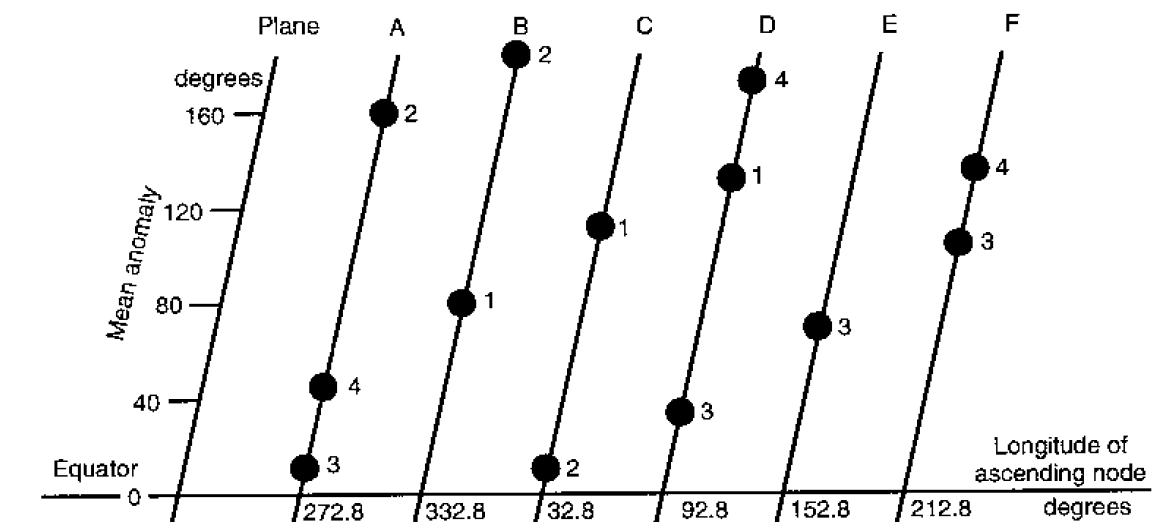
\includegraphics[width=6cm]{./bilder/GPS-SatConstellation.png}    
    \end{minipage}
	
	\subsubsection{control network}
	Die drei Hauptaufgaben des von der USA gestellten Kontrollnetzwerk sind:
	\begin{liste}
    	\item Überwachung der SV-Bewegungen
    	\item Überprüfen des SV-clocks
    	\item Die Zeitsynchronisation der SV
    \end{liste} 
\subsection{Signal Charakteristik\formelbuch{187}}
	\subsubsection{Übersicht}
		\begin{minipage}{9cm}
      		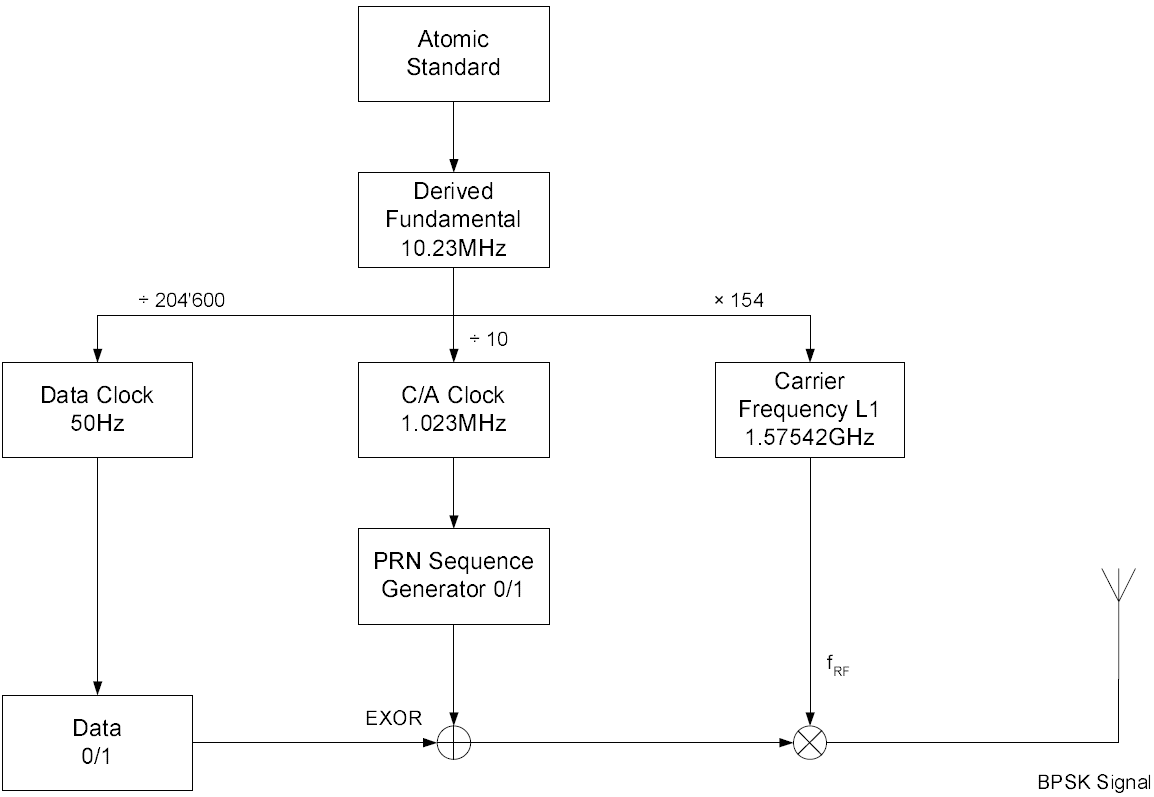
\includegraphics[width=9cm]{./bilder/GPS-Signalaufbau}
        \end{minipage}
		\begin{minipage}{10cm}
        	Alle SV senden auf der gleichen Frequenz. Dadurch muss das
        	Signal CDMA- codiert sein.\\
        	Datensignal: Die Datenrate ist nur 50 bits/s. Für alle Informationen	
        	braucht man 12.5min. Es werden folgende Informationen übertragen:
        	\begin{liste}
            	\item SV- Zeit
            	\item Ephemeriden: genaue Positionsdaten des SV
            	\item almanac: ungefähre Positionsdaten aller SVs
            	\item Zeit Korrektur
            	\item Ionosphäre Daten
            	\item Gesundheitsinformation des SVs
            \end{liste}
		\end{minipage} 
	\subsubsection{PRN Sequenz: Gold code}
		\begin{minipage}{10cm}
        	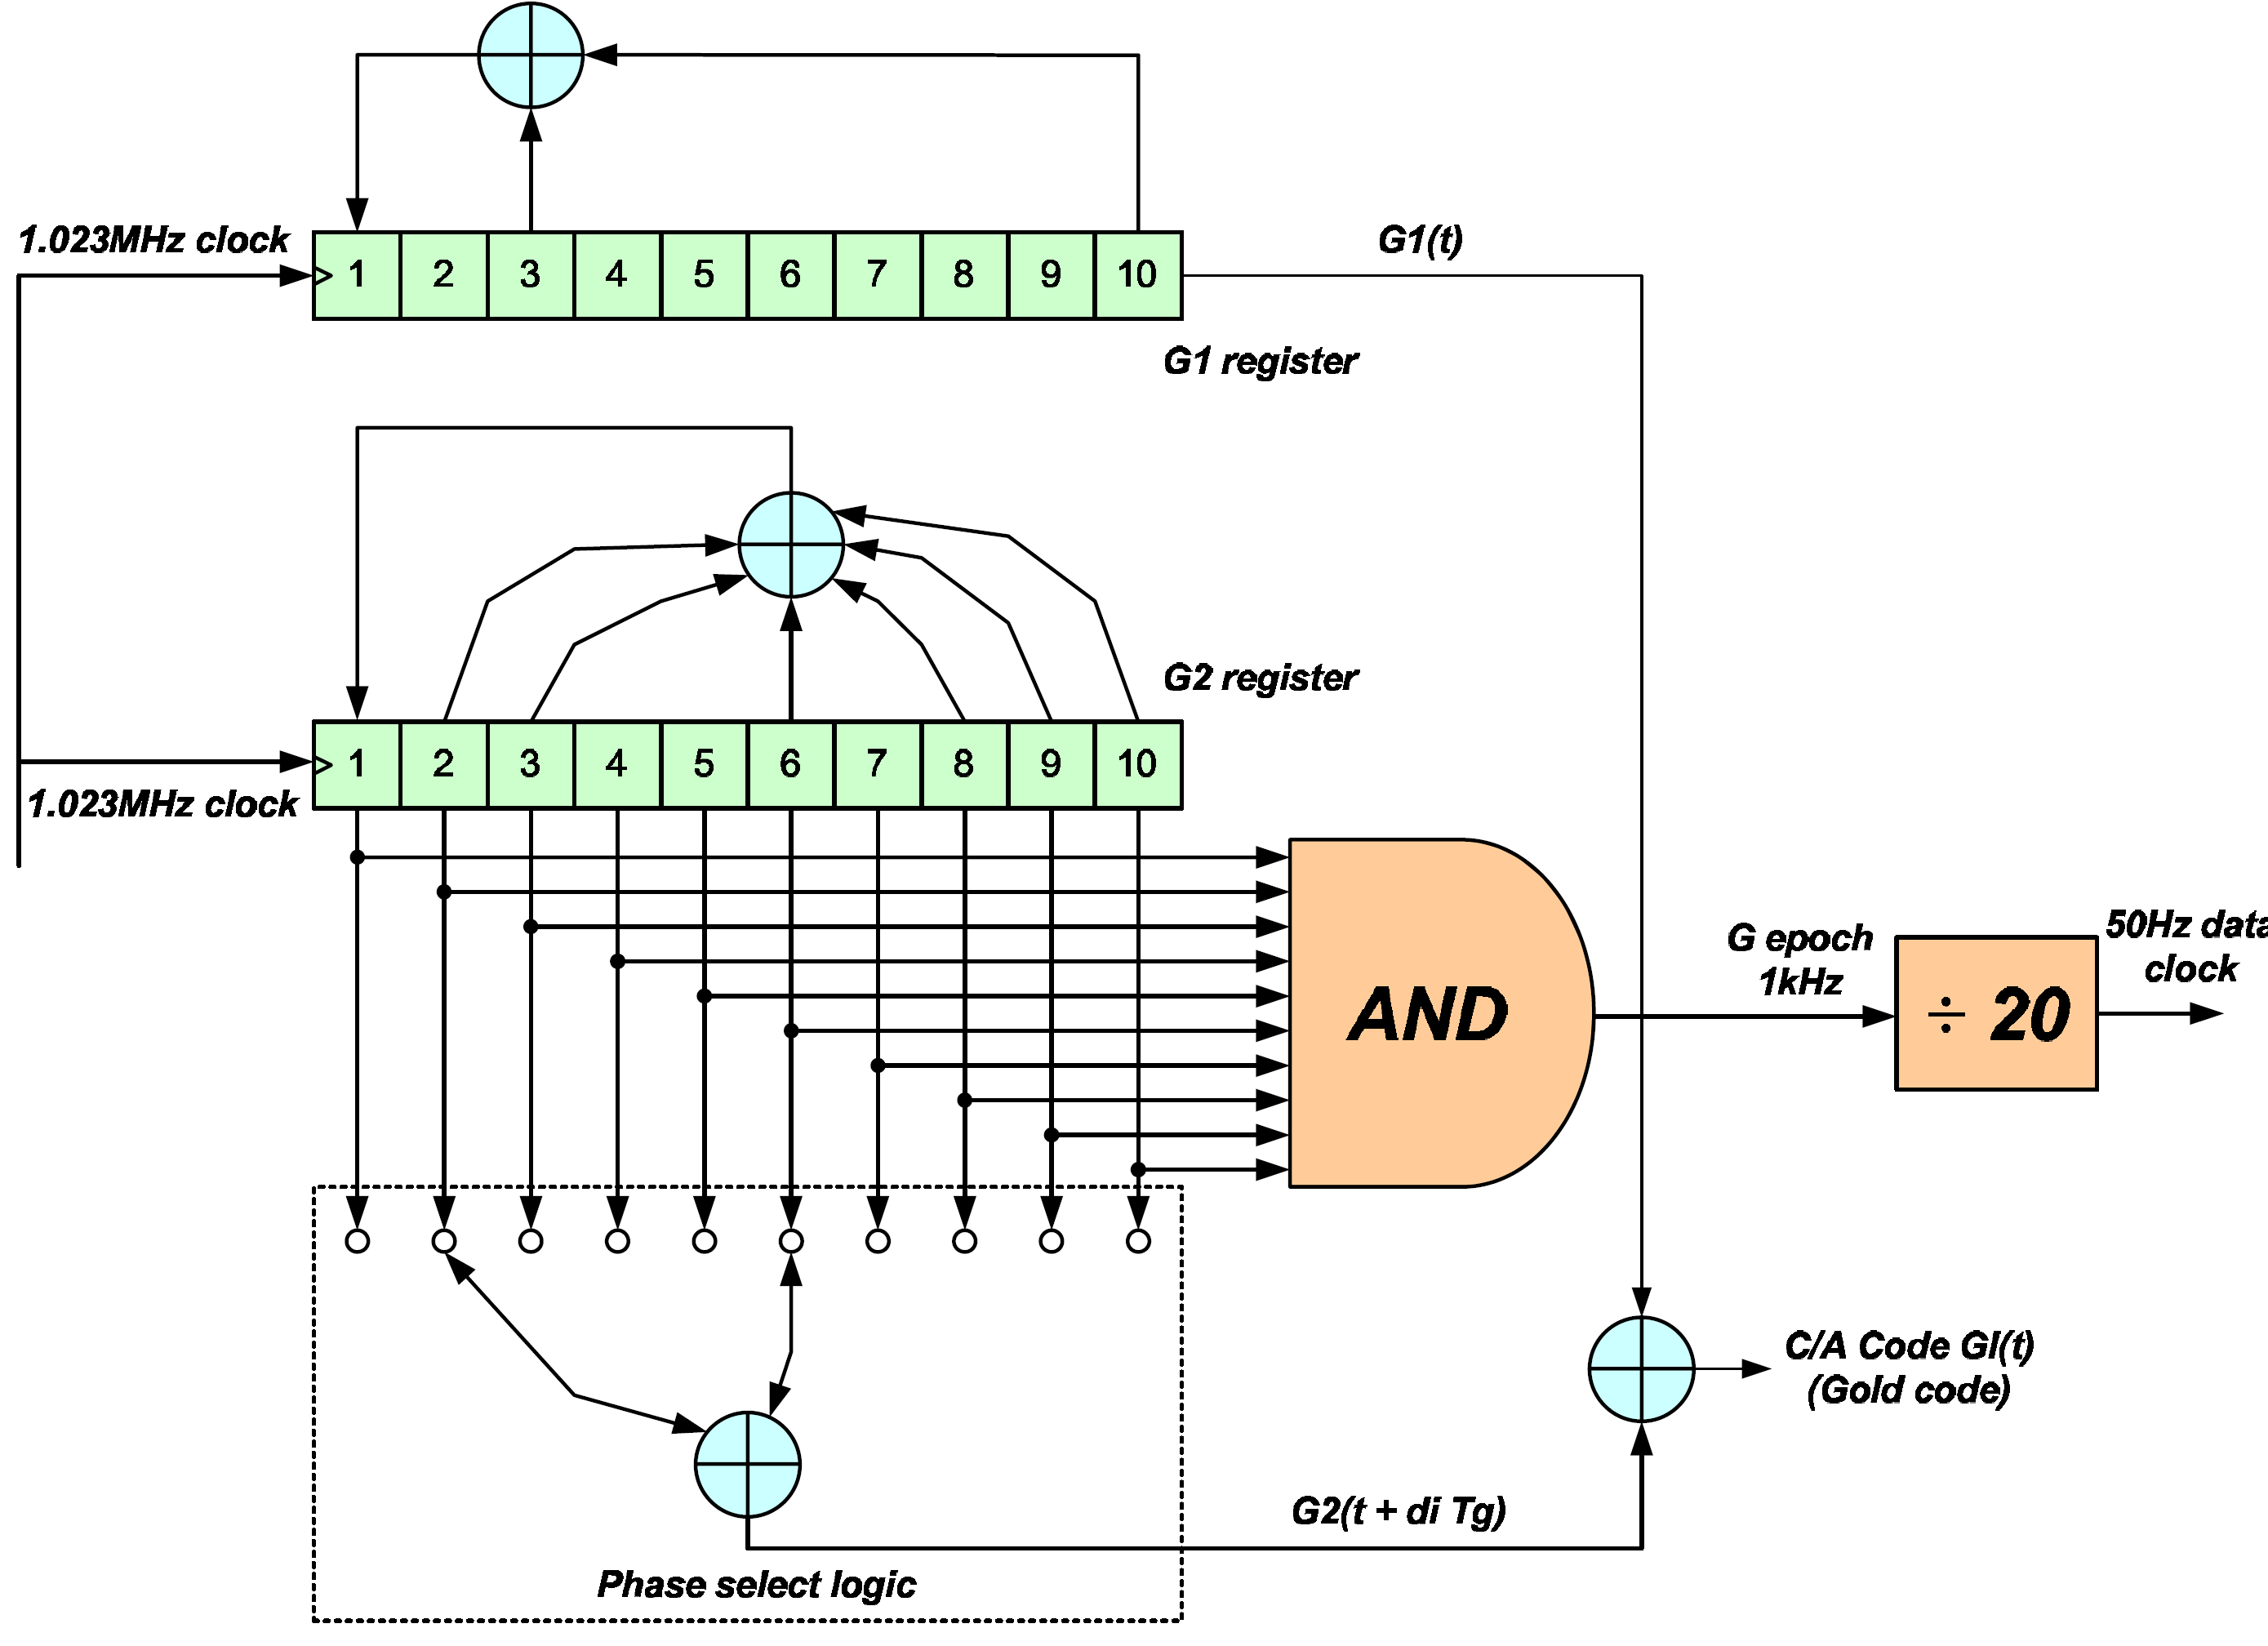
\includegraphics[width=9cm]{./bilder/GPS-Gold.png}
        \end{minipage}
		\begin{minipage}{8cm}
        	Jeder SV hat genau eine Sequenz
        	von $2^n-1=2^{10}-1=1023$ Bits. Dadurch wird die PRN Sequenz alle
        	1ms wiederholt. Pro Datenbit hat es genau 20 Sequenzen, dass heisst es
        	wird jeweils nur ganze Sequenzen mit $\pm$1 multipliziert werden\\
        	Eine Gold- Sequenz wird durch zwei 10 Bit Register erzeugt, welche
        	unterschiedlich mit EXOR rückgekoppelt werden. Beim schlussendlichen
        	Signal wird der Ausgang des ersten Register mit dem verzögerten
        	Ausgang oder durch EXOR verknüpte Bit des zweiten Register verknüpft.
        	Je nach Verzögerung bzw. EXOR- Verknüpfung kann man auf den Satellit
        	schliessen.
        \end{minipage}
			
	\subsubsection{Signalleistung}
		Der free-space loss ist:\\
		$$L [dB] = 147.6 +20\log_{10}(Frequenz)+20\log_{10}(Distanz) = -147.6 +
		20\log_{10}(1.57542\cdot10^9) + 20\log_{10}(2.5785\cdot10^7) = 184.6 dB$$\\
		Die Empfangsleistung ist:\\
		$$P_{\text{rx}} = P_\text{sende} + \text{antenna gain} - \text{free space
		loss} - \text{atmosphere loss} = 43.4 + 13.4 - 184.6 - 2 \approx
		-130\,\text{dBm}$$\\
		Die Rauschleistung ist bei einer Bandbreite $B\approx 1$ MHz:\\
		$$P_\text{Noise}=-174dB+10\log_{10}(B\text{Hz})\approx-114\text{dBm}$$\\
		Das ergibt ein SNR von ca. -14dB. Durch Korrelation kann jedoch die SNR
		theoretisch um einen Faktor von $G=10\log_{10}(1023)=30\text{dB}$
		verbessert werden (sogenanntes Process Gain G).
	\subsubsection{Korrelation}
		\begin{minipage}{6cm}
        	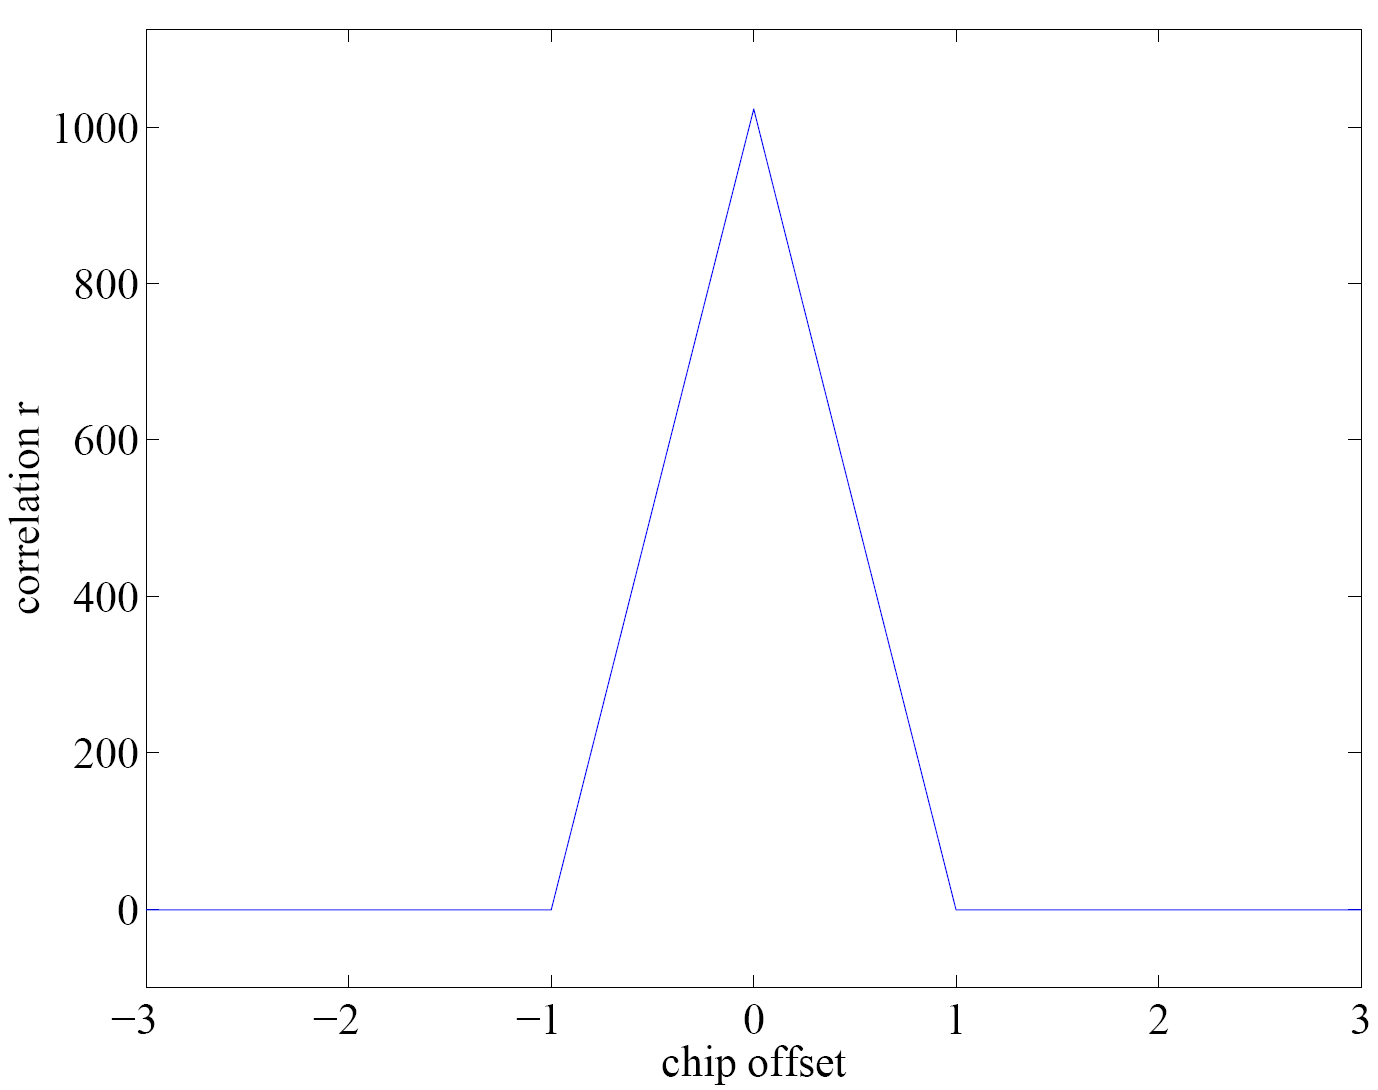
\includegraphics[width=6cm]{./bilder/GPS-Autokorrelation.png}
        \end{minipage}
		\begin{minipage}{6cm}
        	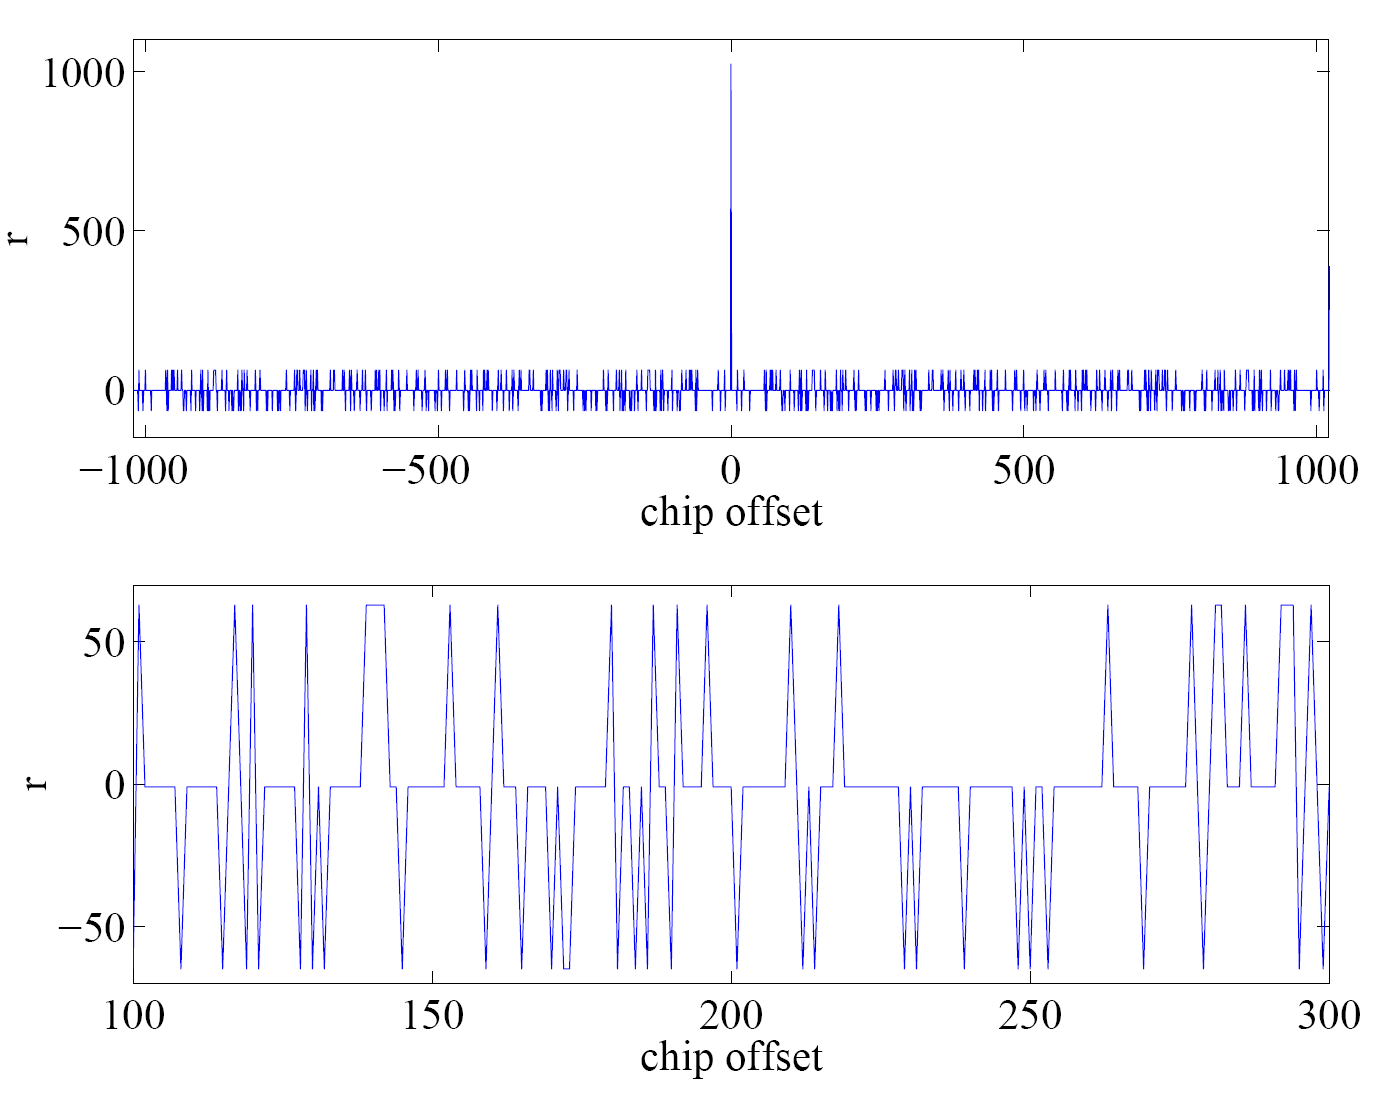
\includegraphics[width=6cm]{./bilder/GPS-Autokorr_Sequenz.png}
        \end{minipage}
		\begin{minipage}{6cm}
        	Der Peak der Autokorrelation ist 1023 hoch. Da eine Sequenz immer eine
        	ungerade Anzahl an Bits hat, ist sonst der Wert bei der
        	Auto- wie auch bei der Kreuzkorrelation -1. Ausserdem können
        	auch die Werte +63 und -65 vorkommen.\\
        	Falls ein Satellitensignal um
        	$20\log_{10}(\frac{1023}{63})=23.9\text{dB}$ stärker ist, kann eine
        	Verwechslung auftreten.
        \end{minipage}

\newpage

\subsection{Empfänger Architektur\formelbuch{194}}
	\begin{minipage}{10cm}
		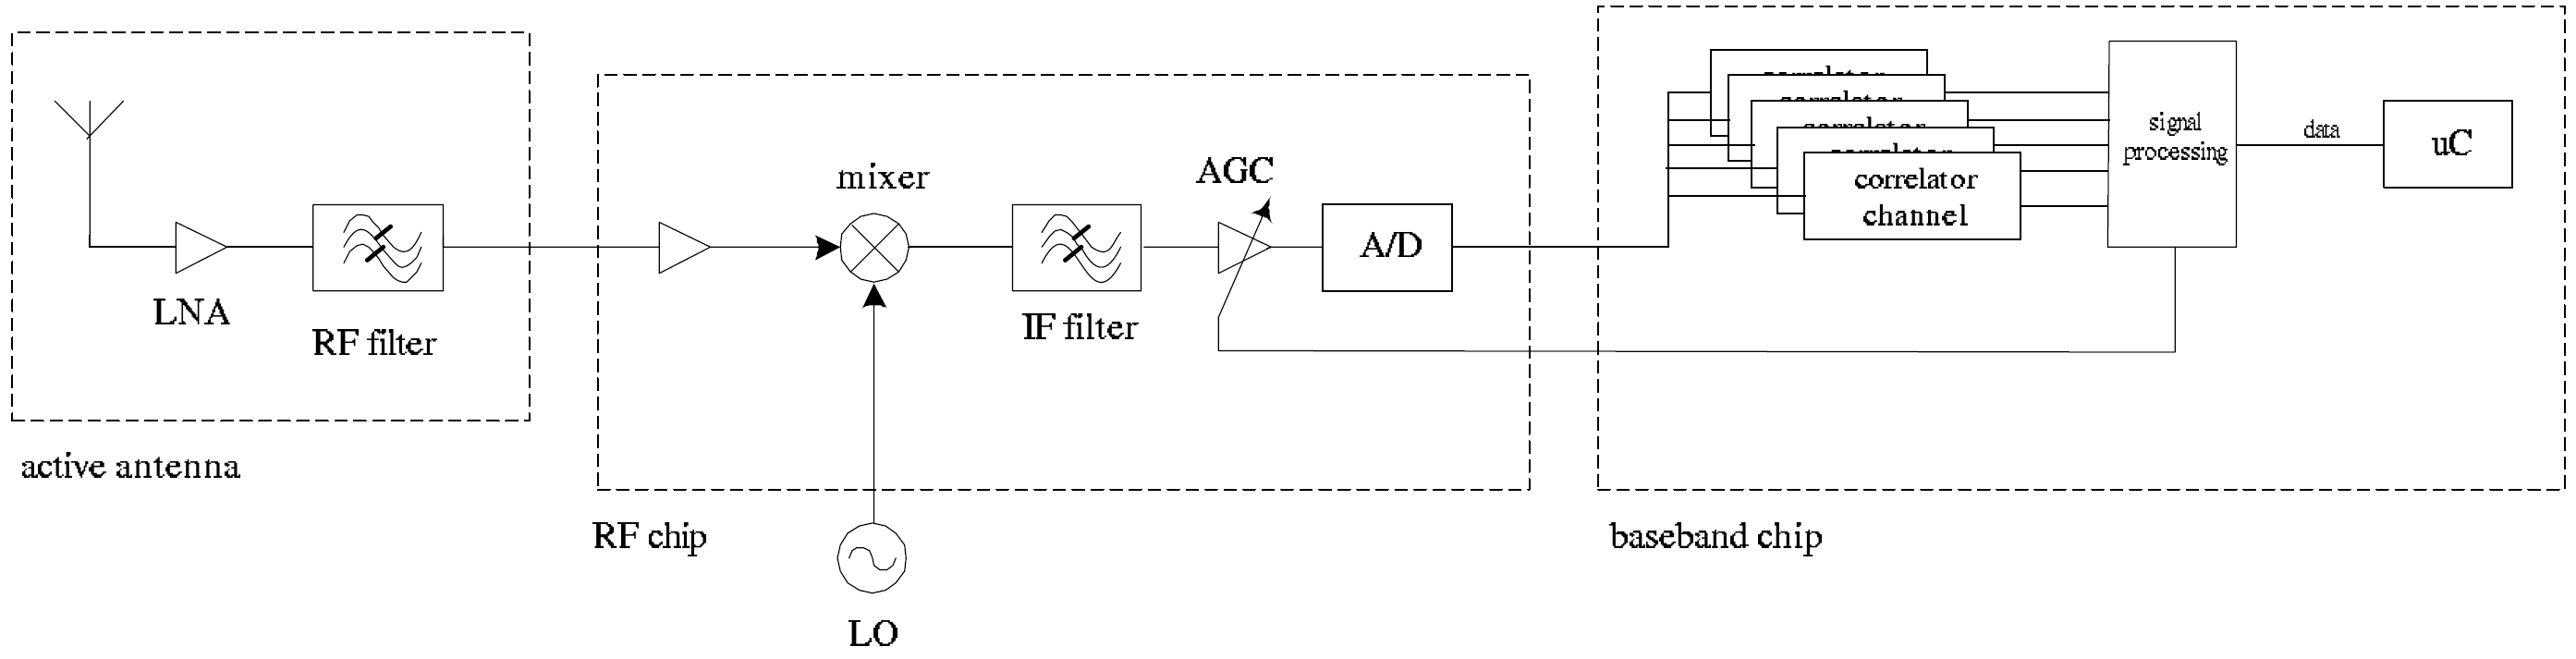
\includegraphics[width=10cm]{./bilder/GPS-Empfangsarchitecture.png}
	\end{minipage}
	\begin{minipage}{8cm}
    	\textbf{Antenna}: Die Antenne muss zirkular polarisiert (Gegenuhrzeiger)
    	sein(RHCP). Um nur das normale Band empfangen zu können (1.57542GHZ),
    	braucht sie nur eine kleine Bandbreite. \\
    	\textbf{LNA}: Meist wird dieser direkt im Antennen Gehäuse integriert.
    \end{minipage}\\
	\textbf{AGC}: Im Gegensatz zu anderen wireless Anwendungen wird hier der
    	AGC nur verwendet, um die Unterschiedlichen LNA auszugleichen (zB. wenn
    	keine bzw. eine aktive Antenne gebraucht wird)\\
    \begin{minipage}{8cm}
    	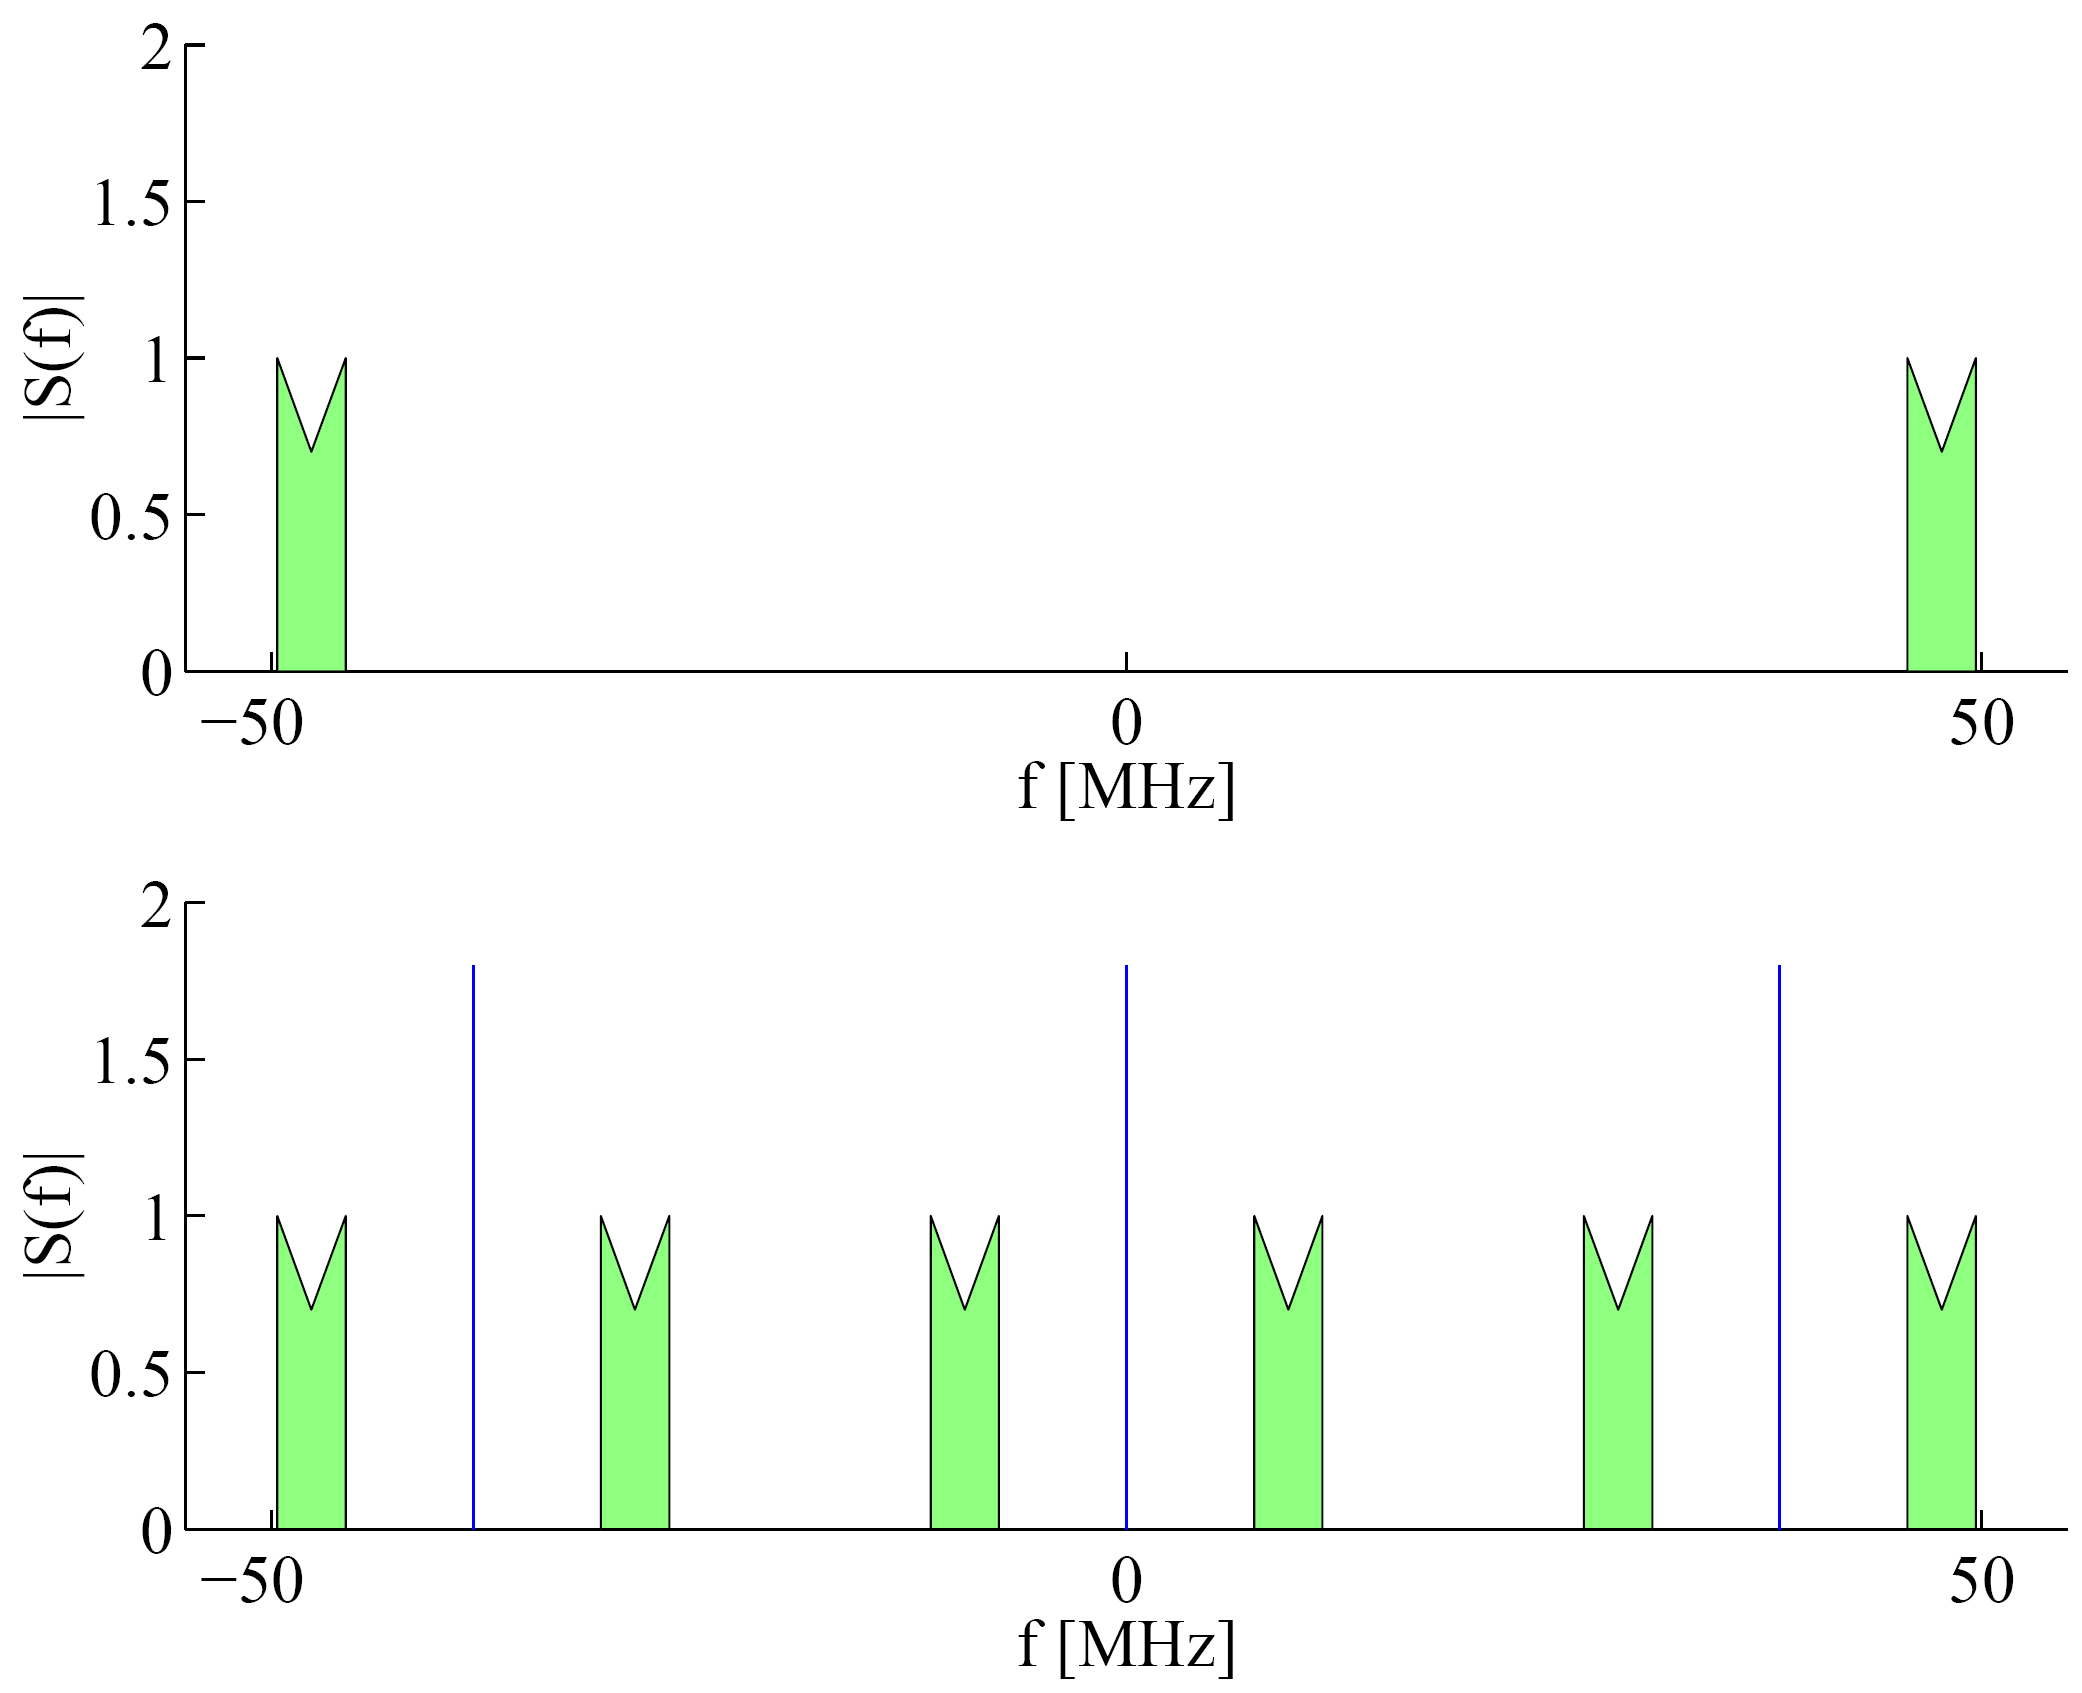
\includegraphics[width=6cm]{./bilder/GPS-Downsampling.png}
    \end{minipage}
	\begin{minipage}{9cm}
	    \textbf{ADC}: Wenn man das bekannte Nyquist-Gesetz erweitert zu $2B\leq
	    f_s$ kann man ein bandbegrenztes Signal mit dem Abtasten auch noch
	    runtermischen. Dafür muss noch folgende Bedingung zur Abtastfrequenz
	    eingehalten werden:\\
	    $$\frac{2f_u}{n}\leq f_s\leq\frac{2f_l}{n-1}\text{ mit }|
	    f_l=IF-\frac{B}{2};f_u=IF-\frac{B}{2}$$
	   	
    \end{minipage}\\
	IF von 47.65MHz; $f_s=38.194$MHz ergibt $IF_{Digital}=47.65-38.194=9.456$MHz
    
\subsection{GPS und die Relativitätstheorie\formelbuch{202}}
	\begin{minipage}{10cm}
    	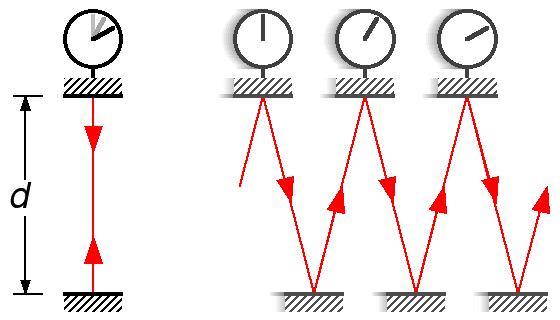
\includegraphics[height=4.5cm]{./bilder/GPS-Relativitaettheory.png}\\
    	Lichtuhrversucht für die Spezielle Relativitätstheorie
    \end{minipage}
	\begin{minipage}{8cm}
		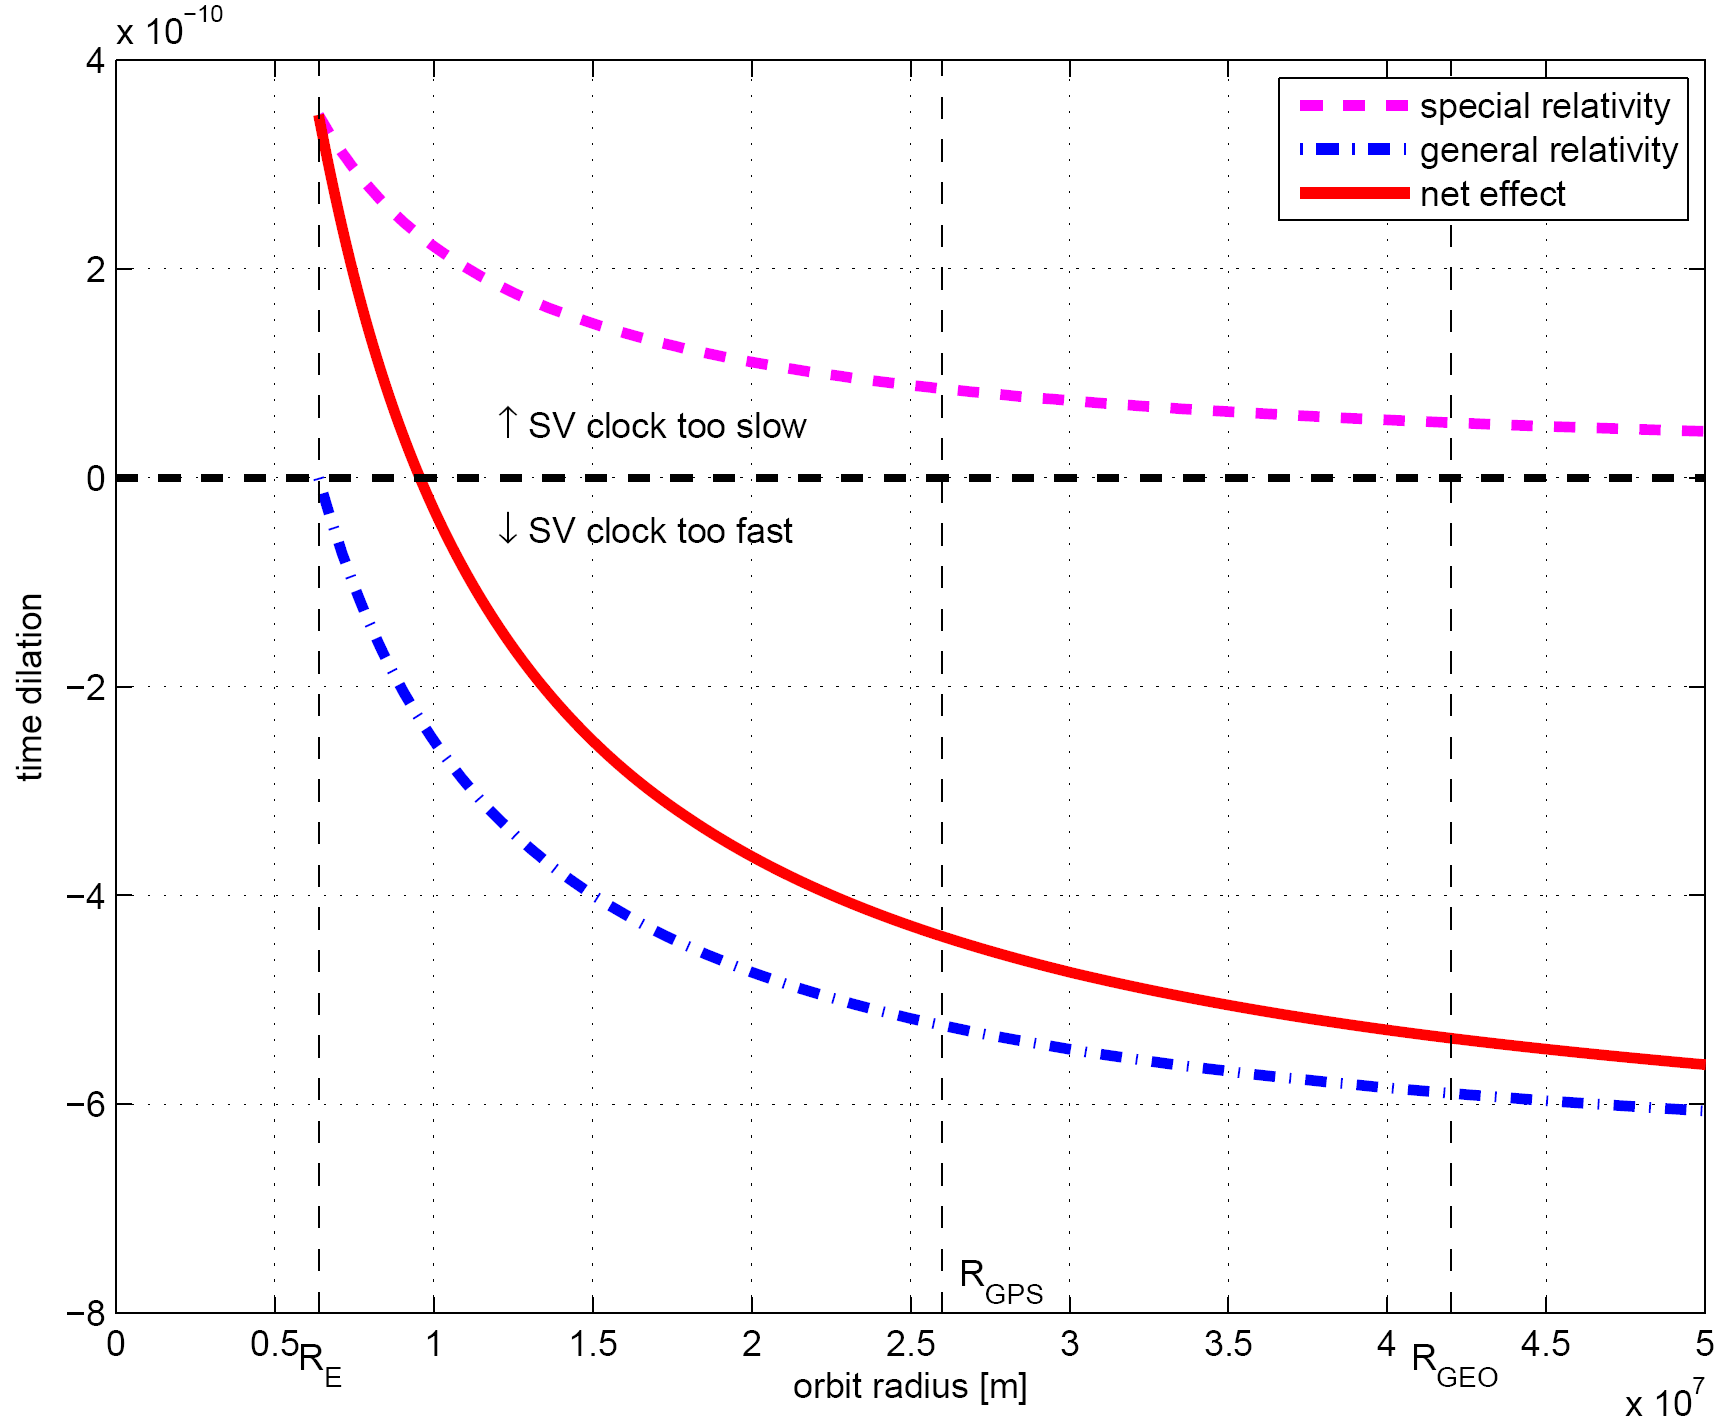
\includegraphics[height=5cm]{./bilder/GPS-ZeitKorrektur.png}\\
		Übersicht der beiden wirkenden Zeitveränderungen
	\end{minipage}\\ \\
	Das Licht legt die Strecke d zurück löst einen Impuls aus und wird
	reflektiert, etc. (\textbf{spezielle Realtivitätstheorie}) \\
	$v=konst.\Rightarrow$ Zeit des bewegenden Objekts ist langsamer da eine
	grössere Strecke zurückgelegt werden muss 
	$ t'_{bew} = \frac{t_{ruh}}{\sqrt{1 - \frac{v^2}{c^2}}}$\\
	Für einen Satelliten ergibt sich dann:
	$t_{SV_1}= t_{Erde} \frac 1{\sqrt{1-\frac{g}{c^2}\cdot \frac{R_E^2}R}}$\\
	Die \textbf{generelle Relativitätstheorie} besagt, dass sich ein Clock
	langsamer ist, wenn er in einem Gravitationsfeld ist.\\
	$t_2 = t_0 \frac 1{\sqrt{1-\frac{2GM}{Rc^2}}} 
  	= t_0 \frac 1{\sqrt{1-\frac{g}{c^2}\cdot 2\frac{R_E^2}R}}$; 
  	$t_{SV_2}= t_E \frac{\sqrt{1-\frac{g}{c^2}\cdot 2 R_E }}
    {\sqrt{1-\frac{g}{c^2}\cdot 2\frac{R_E^2}R }}$\\
    Der totale Effekt ist, dass der Quarz des Satelliten mit nur
    10.229999995433MHz anstatt den 10.23MHz laufen muss.
    
%\newpage    
\subsection{Acquisition and Tracking\formelbuch{206}}

	\begin{center}
    	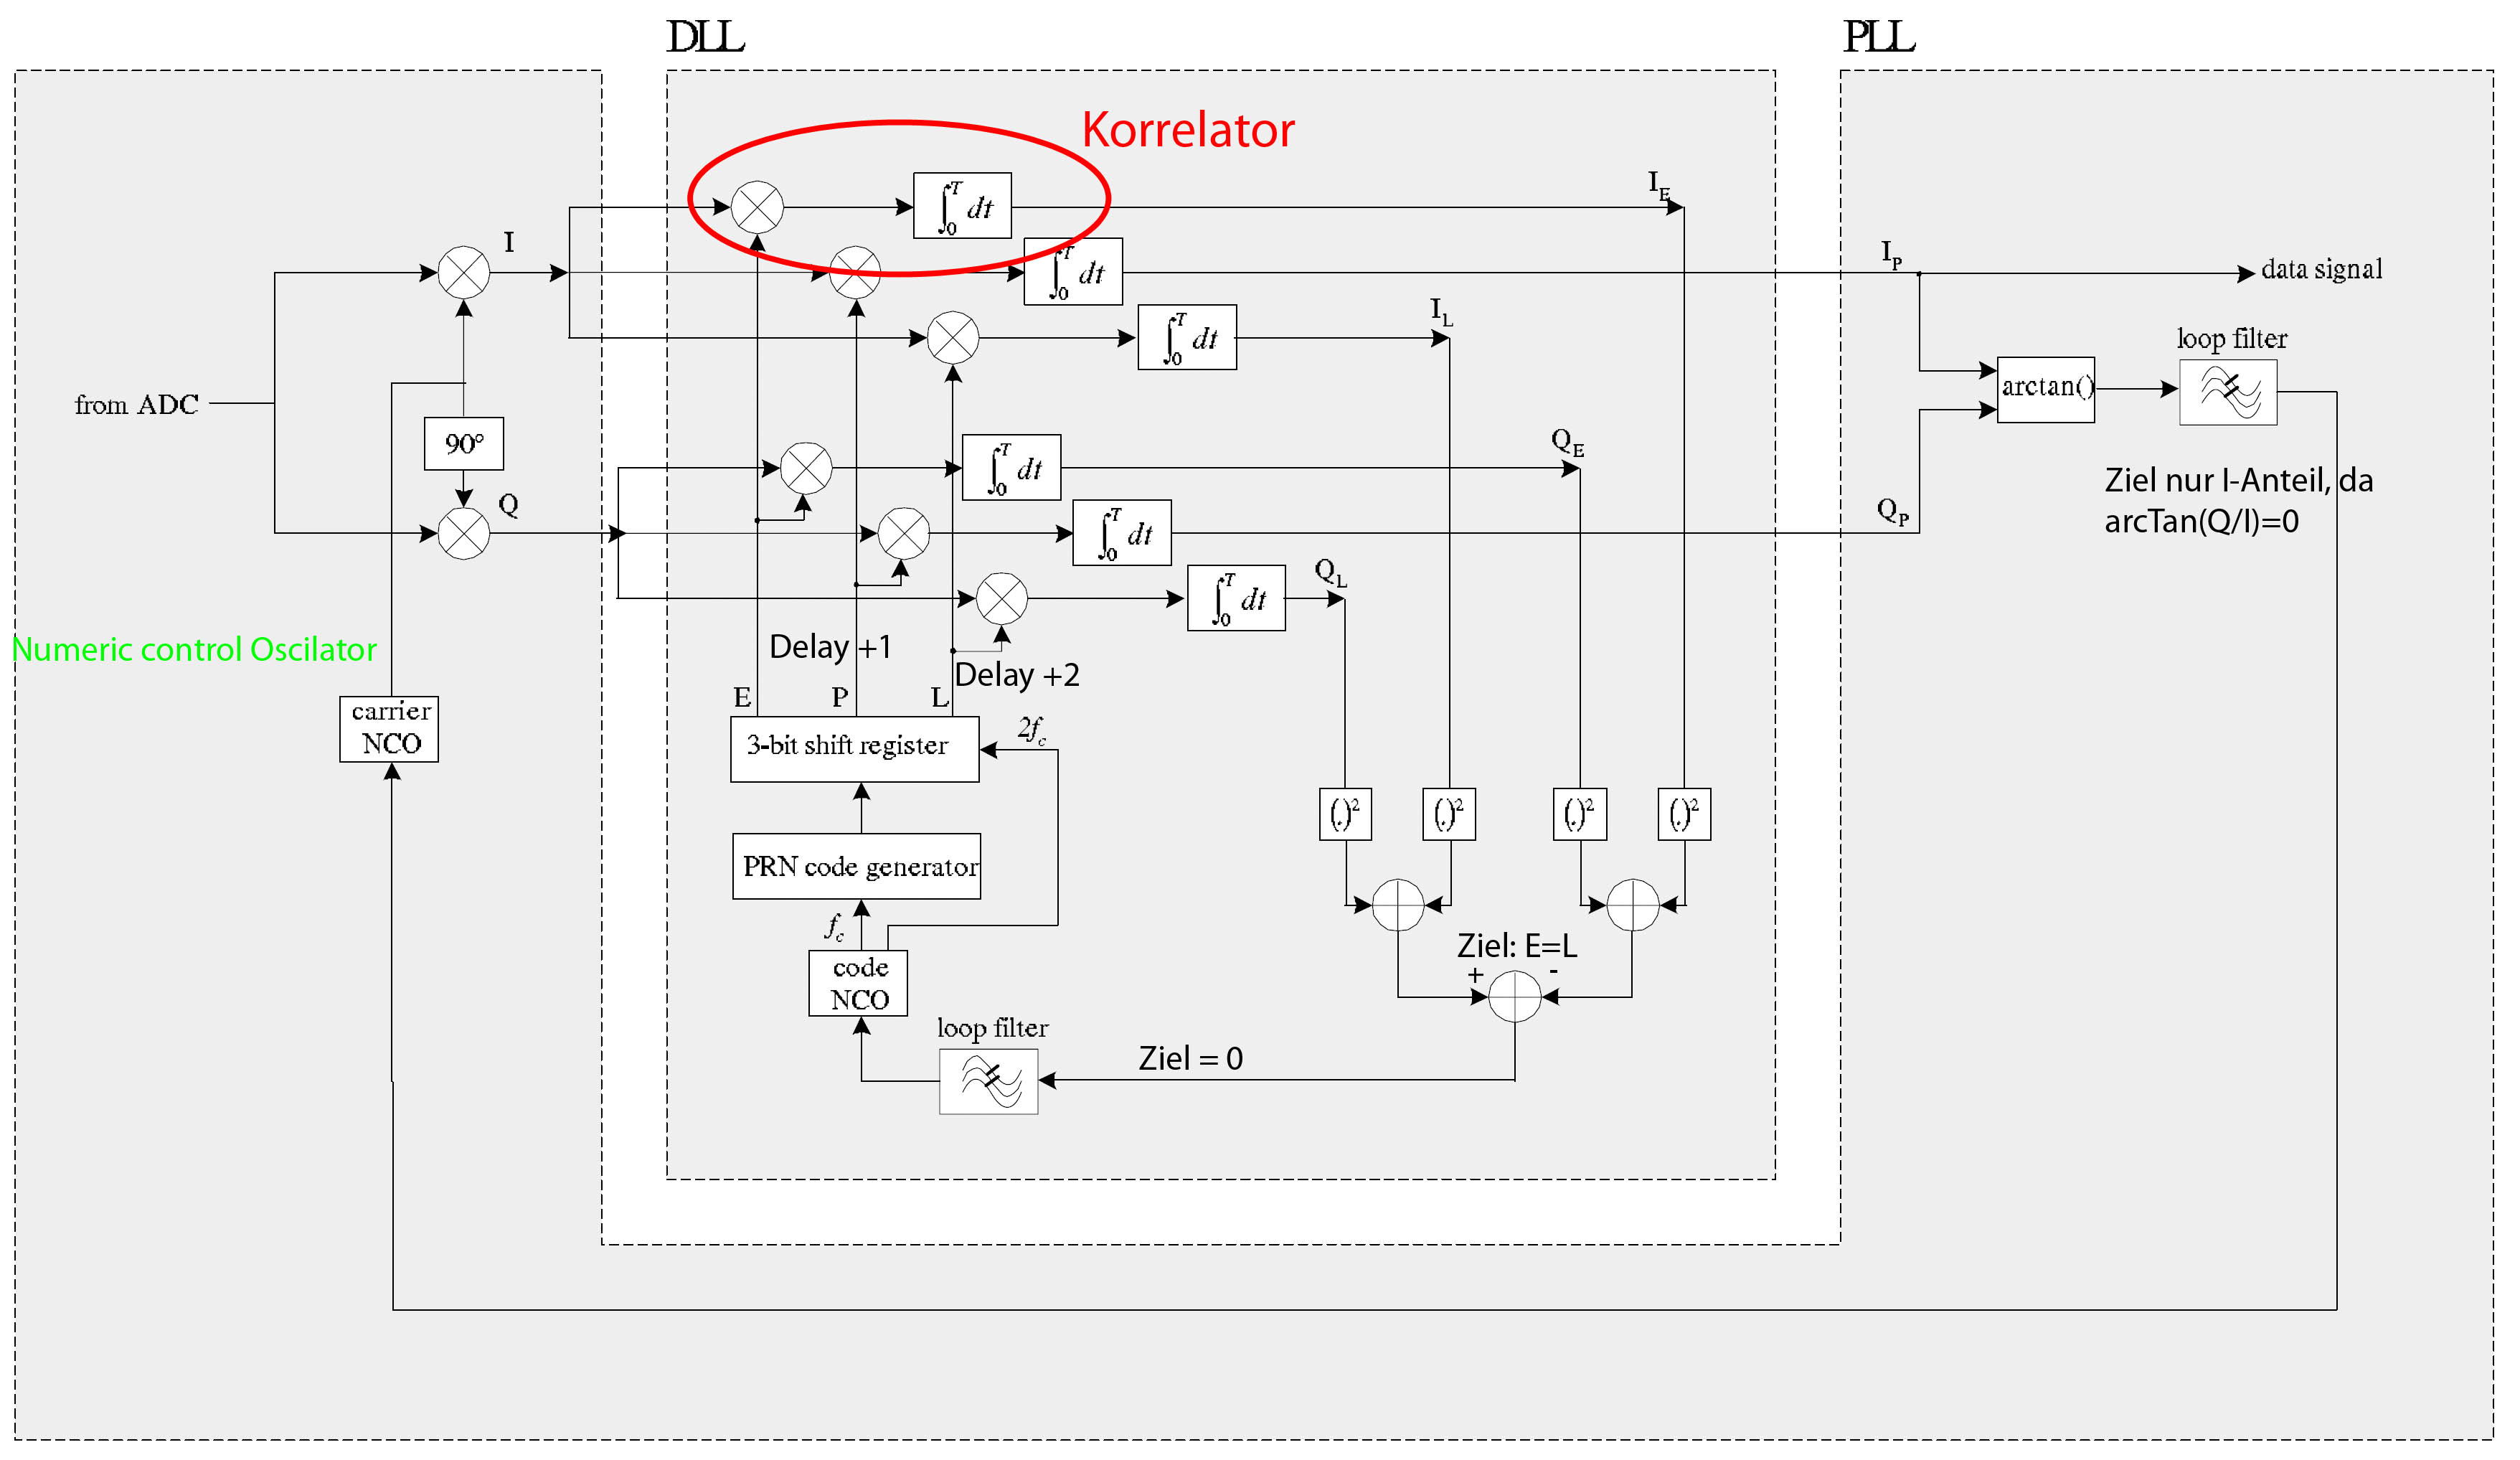
\includegraphics[width=14cm]{./bilder/GPS-Phasenlock.jpg}\\
    \end{center}

	Um die Satelliten zu finden muss in 3 Dimensionen gesucht werden:
	\begin{liste}
    	\item SV nummer: 	1 bis 28 (Anz: 28)
    	\item Code Phase: 	0 bis 2045 (halbe Bitbreite) (Anz: 2046)
    	\item Frequenz:		-35kHz bis +35kHz (Da ca 20ppm = 30kHz und $\pm$ 5kHz
    	Dopplershift in je 500Hz Schritten) (Anz:141)
    \end{liste}
	Das ergibt ohne jegliches Vorwissen für jeden Satellit $N=2046\cdot
	141=288486$ Möglichkeiten.\\
	Für die Auswertung muss $s=I_P^2+Q_P^2$ gerechnet werden (Korrelation) und eine
	Peakdetection vorgenommen werden.
	
	Bei guter Versorgung dauert die Time-To-First-Fix (TTFF) im Minimum 18\,s und im Maximum 36\,s.
	Das kommt durch den Aufbau der Navigationsnachricht zustande. \\
	\begin{minipage}{14cm}
	    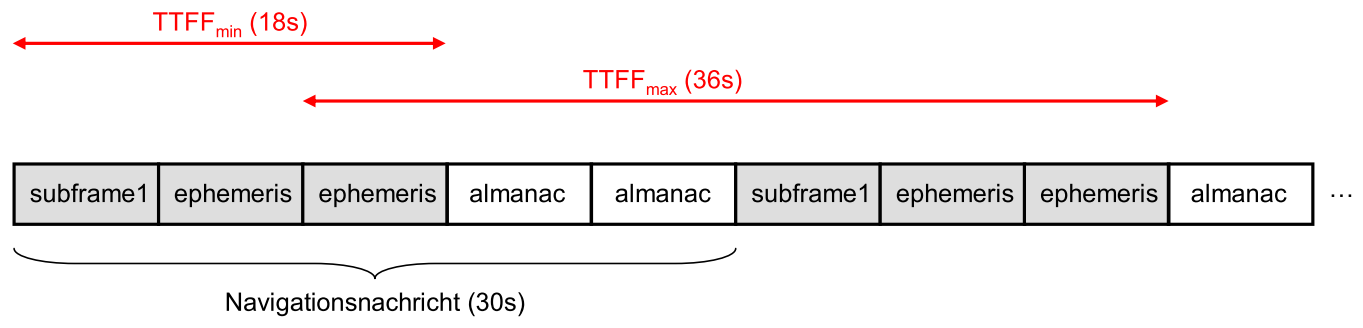
\includegraphics[width=14cm]{./bilder/GPS-ttff.png}
    \end{minipage}
	
	Mit Hilfe von Assisted GPS (A-GPS) kann die TTFF drastisch verkleinert werden (auf ca. 1-3\,s). Beim A-GPS werden die 
	Ephemeris Daten auf einem Referenz Location Server gespeichert und in sehr schnellen Zyklen gebroadcastet (z.B. via GPRS/UMTS).
	
\subsubsection{Chip resolution}
	\begin{minipage}{10cm}
	    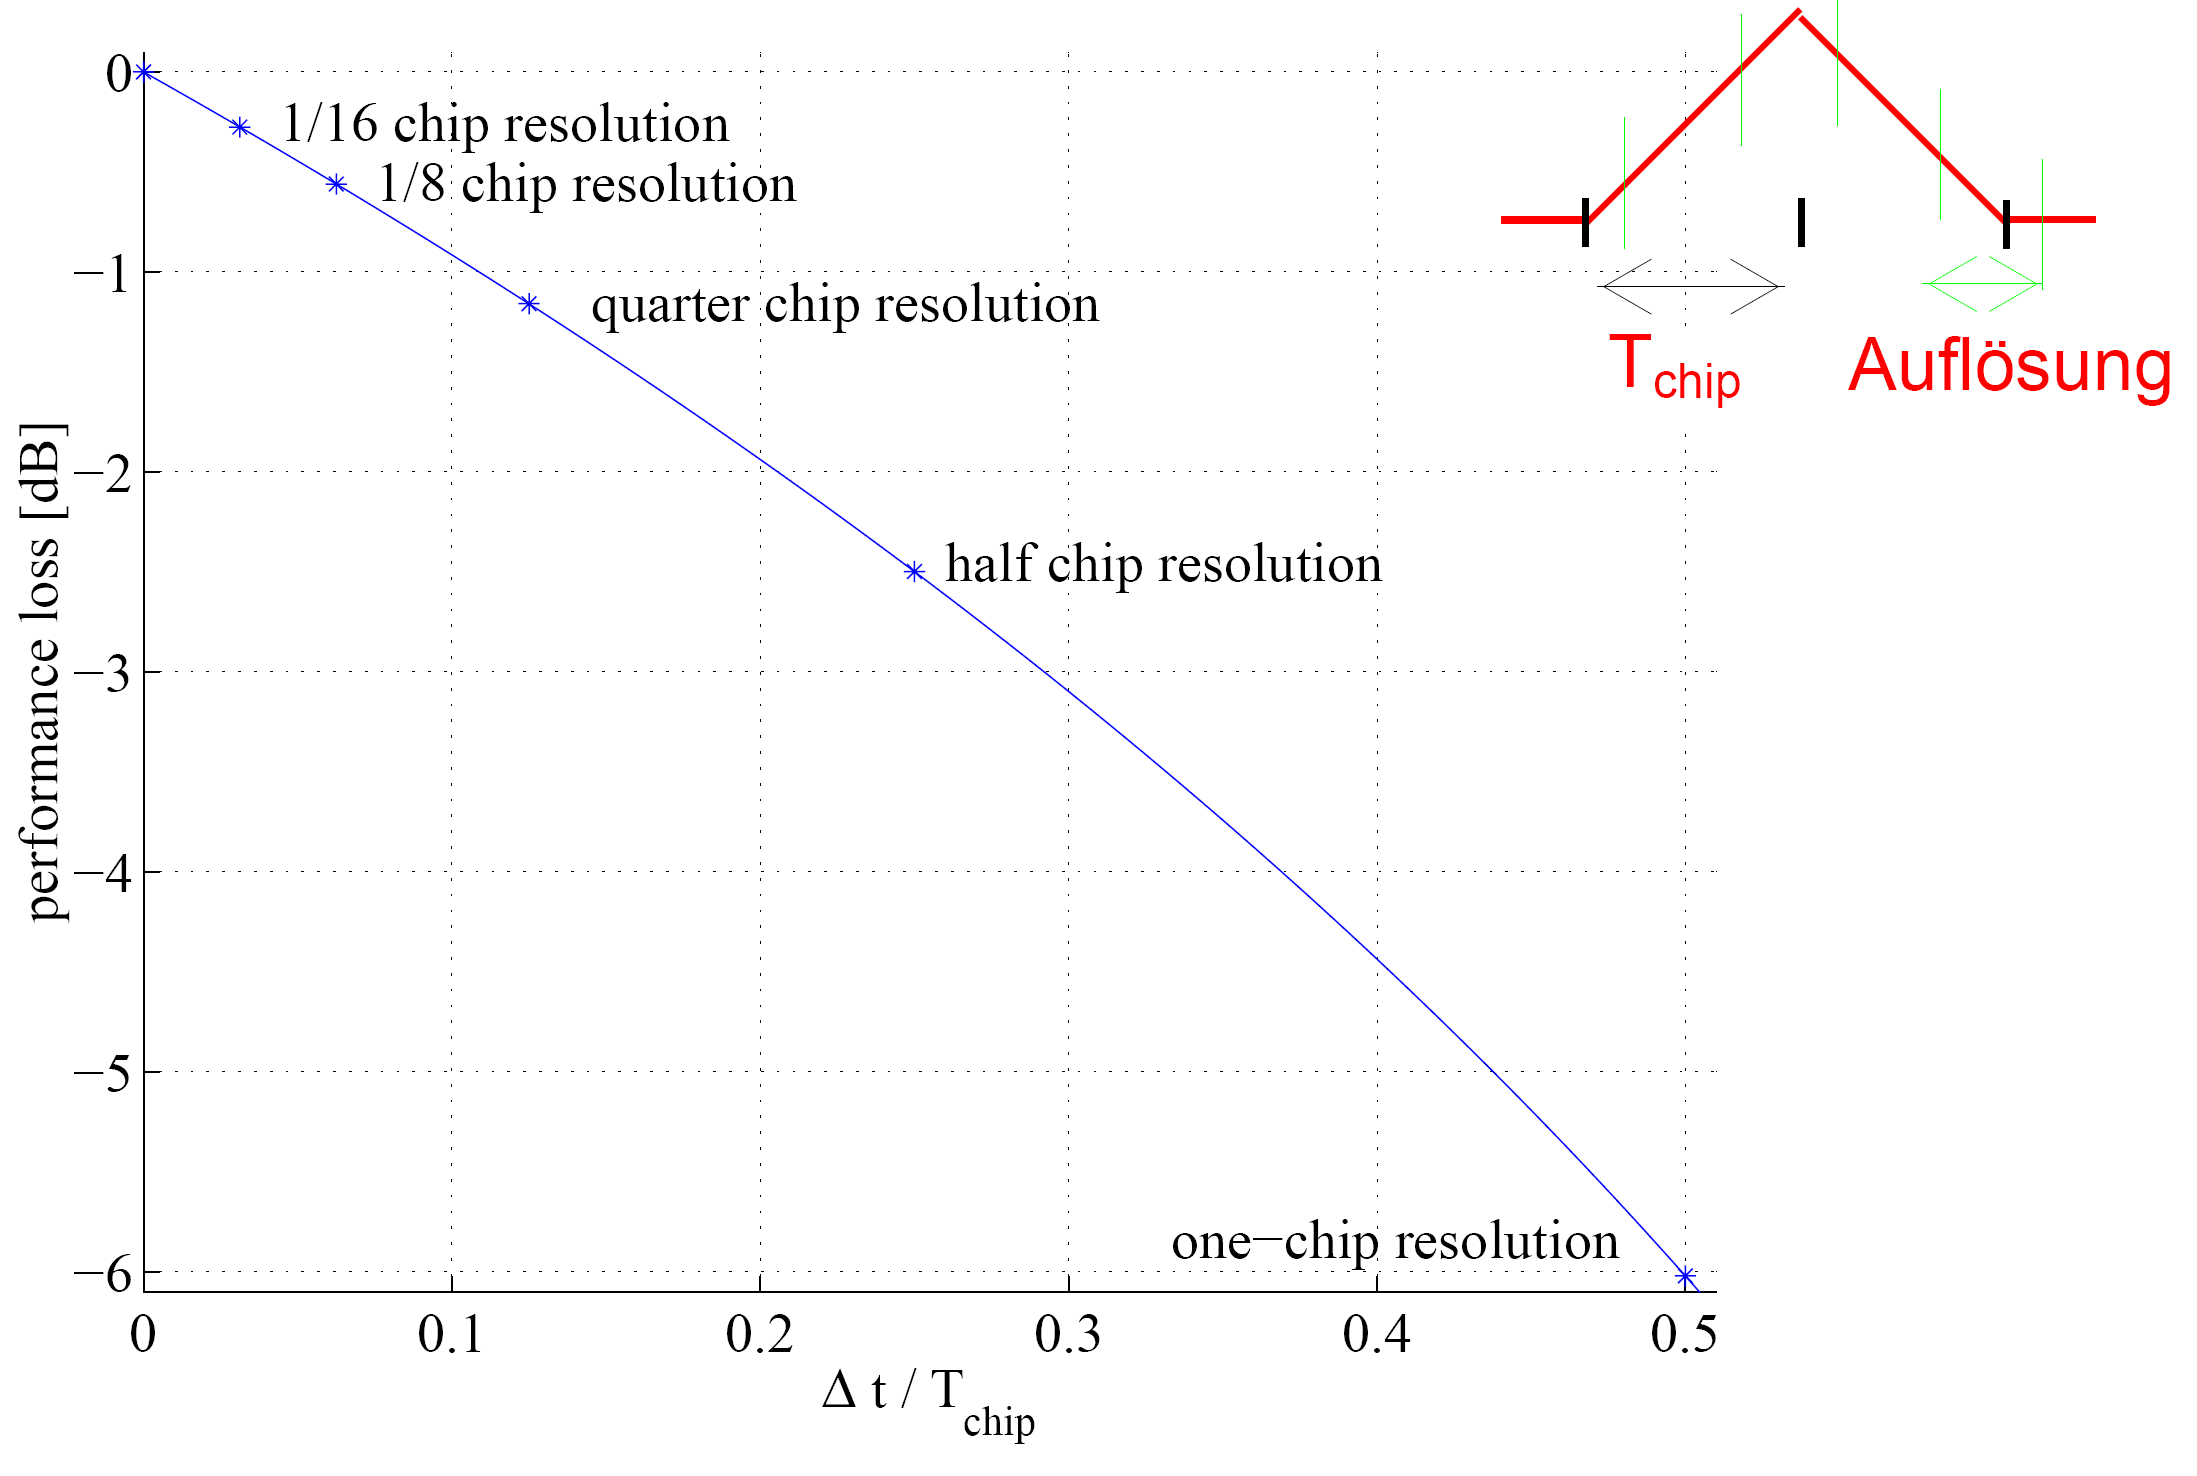
\includegraphics[width=8cm]{./bilder/GPS-ChipResolution.png}
    \end{minipage}
	\begin{minipage}{8cm}
    	Da die Phase nicht genau bekannt ist, treten bei der Detektion des
		Spitzes der Autokorrelation Verluste auf, da nicht mehr das Maximum erwischt
		wird.\\
		$\text{loss [dB]}= 20 \log_{10}\left(1-\frac{|\Delta
		t|}{T_{\mathrm{chip}}}\right)$\\
    \end{minipage}
\subsubsection{Frequenz resolution}
	\begin{minipage}{8cm}
    	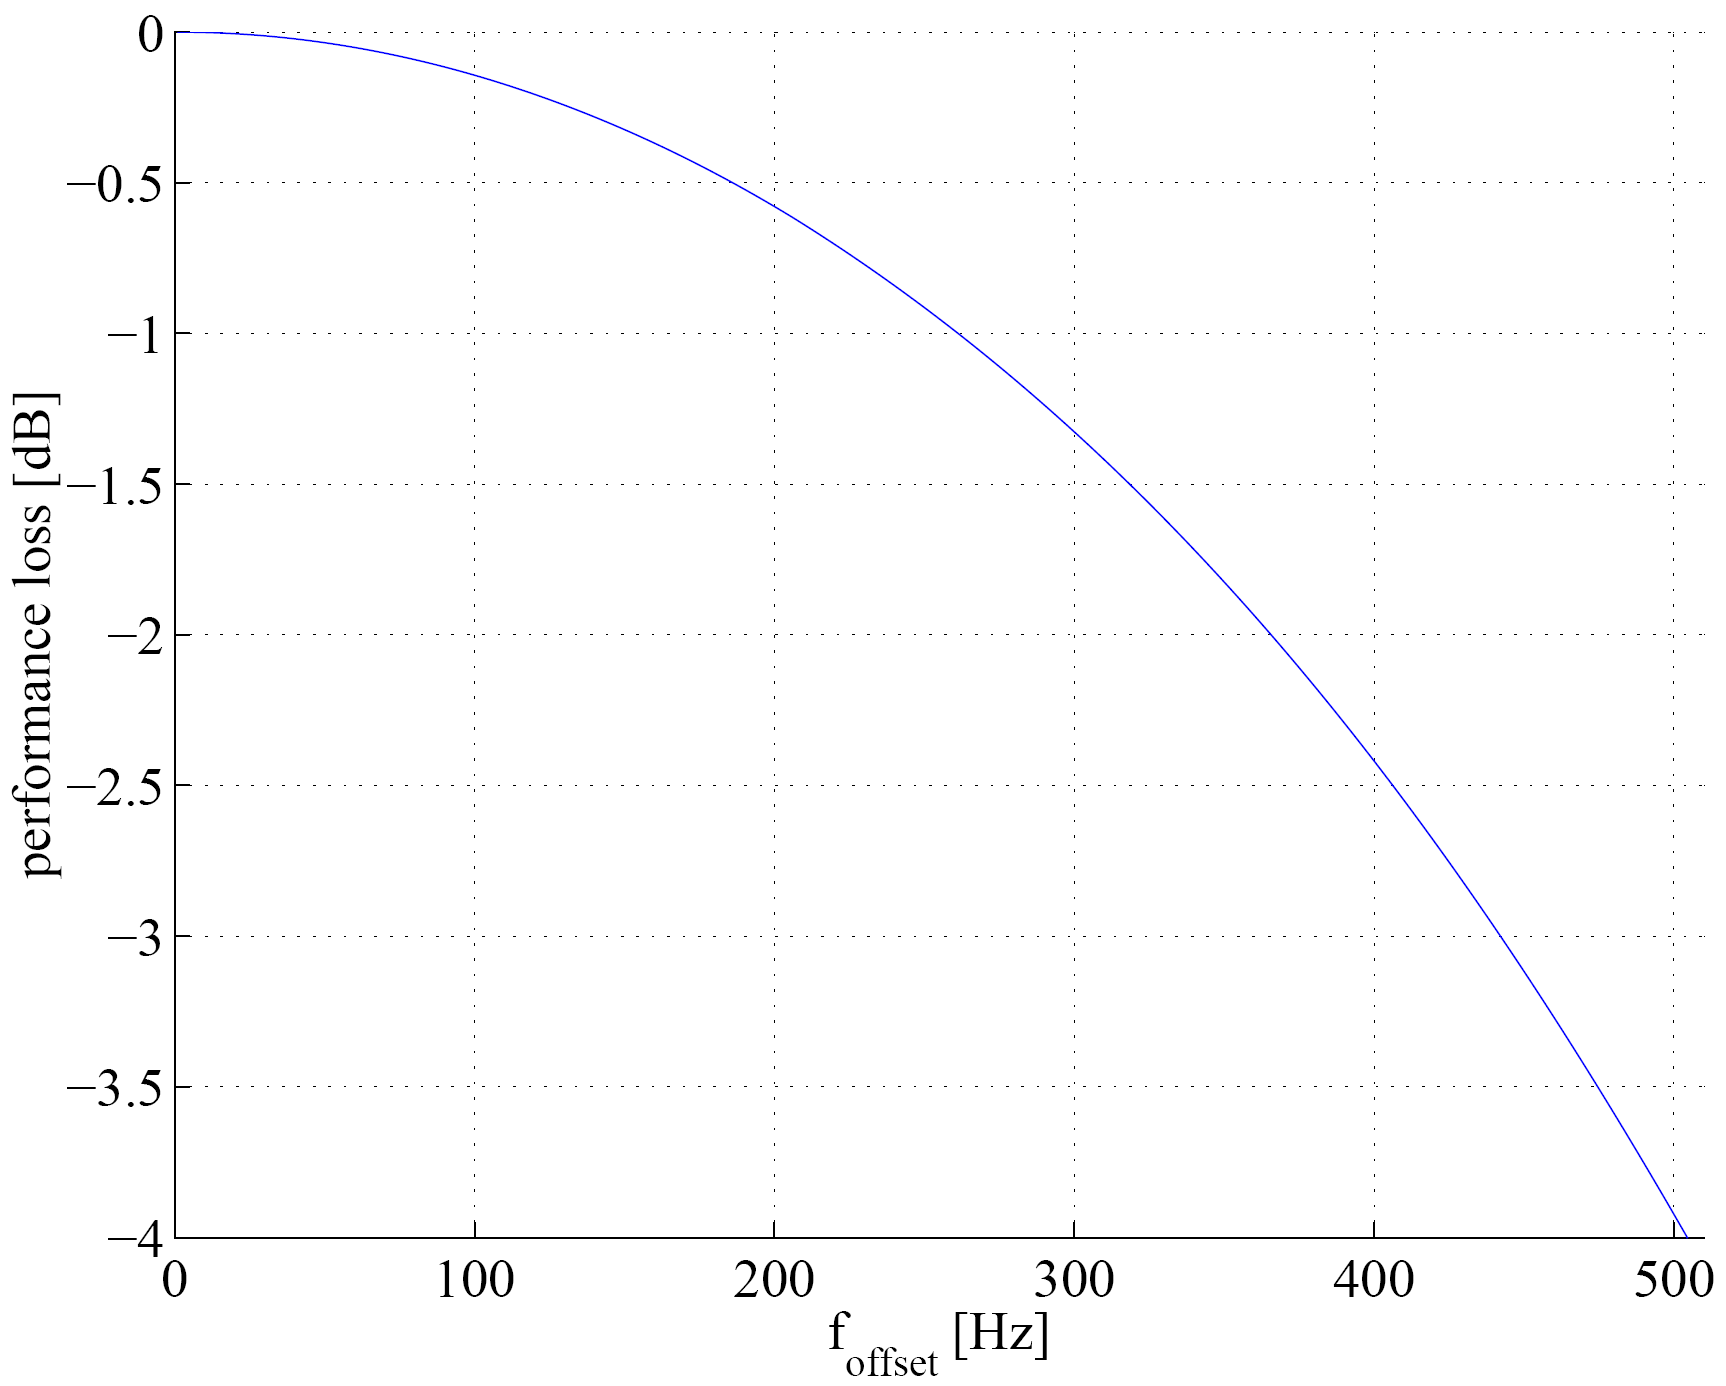
\includegraphics[width=6cm]{./bilder/GPS-FrequenzResolution.png}
    \end{minipage}
	\begin{minipage}{10cm}
	    Bei einem unbekannten Doppler Shift und einer unbekannten Frequenzabweichung
		treten in der Integration Verluste auf.\\
		$\text{loss [dB]}= 20 \log_{10} \frac{\sin(\pi f_{\mathrm{offset}}T)} {\pi
		f_{\mathrm{offset}}T}$\\
     	Grafik links zeigt den Verlust nach der Integration von einer Sequenz
     	(1ms).
    \end{minipage}
\subsubsection{AD conversion with N-bit resolution \formelbuch{210}}
	Die Verluste eines 1-Bit Quantisierer beträgt ca. 2dB. Die eines 1Bit NCO ca.
	1dB.

\subsection{Leistungsfähigkeit und Interferenzen\formelbuch{214}}
	Die Genauigkeit der Positionsmessung wird von folgenden Parameter beeinflusst:
	\begin{liste}
    	\item globale Position (über den Polen hat es eine schlechte
    	Satellitenabdeckung)
    	\item lokale Position (grosse Gebäude in der Nähe, im Thal, etc nur wenige
    	SV sind in Sicht)
    	\item schnelle Bewegung des Users (bei schwachen Signalen sind lange
    	Korrelationen nötig, welche mit den Bewegungen schwieriger werden)
    	\item Komplexitität des Empfängers (Preis/Qualität)
    	\item Andere Einflüsse (zB. Störsender \formelbuch{216})
    	\item Reduktion der Ephemeridenauflösung (5m)
    	\item Brechung der Tropo-/Ionosphäre (siehe\formelbuch{215})
    	\item Mehrpfadfortpflanzung (Problem von Indoor-Anwendungen da Reflektionen
    	etc.)
    	\item schlechte Geometrie von Satelliten
    \end{liste}

\subsection{Dopplereffekt \formelbuch{217}}
\begin{tabular}{lll}
\parbox{5cm}{
    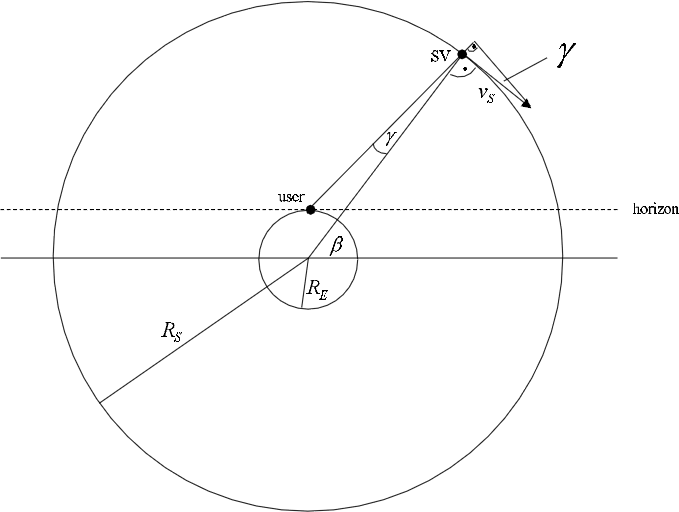
\includegraphics[width=5cm]{./bilder/gps-doppler-constellation.png}}
& \parbox{7cm}{
    $v_{\text{Doppler}} = v_{\text{SV}} R_E\dfrac{\cos \beta}{\sqrt{R_E^2+R_S^2
    -2R_ER_S \sin \beta }}$\\
    $f = \dfrac{v}{c} f_{\text{RF}}$ \\ \\
    $v_{\text{SV}} = 3.8704\frac{km}{h} = 1.0751\frac{m}{s}$ \\
    $R_E = 6378.1363km, R_S = 26561.75km$}
& \parbox{6cm}{
    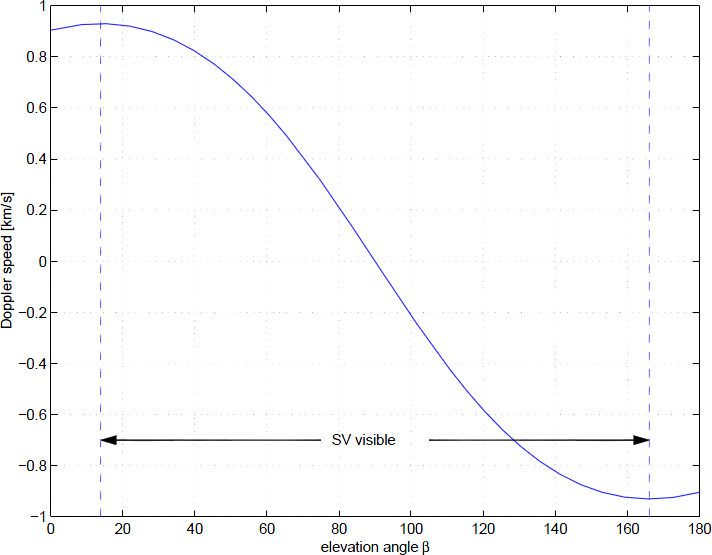
\includegraphics[width=6cm]{./bilder/gps-doppler-speed.png}}
\end{tabular}

\subsection{Navigation\formelbuch{220}}
	Nachdem die SV- Informationen und somit die Zeitdifferenz und
	Satellitenposition entschlüsselt sind, kann die Position wie folgt berechet
	werden:
	$$\rho_1=\sqrt{(x_1-x_{\text u})^2+(y_1-y_{\text u})^2+
                (z_1-z_{\text u})^2}+ c\tau ,  $$
  	$$\rho_2=\sqrt{(x_2-x_{\text u})^2+(y_2-y_{\text u})^2+
                (z_2-z_{\text u})^2}+ c\tau , $$
  	$$\rho_3=\sqrt{(x_3-x_{\text u})^2+(y_3-y_{\text u})^2+
                (z_3-z_{\text u})^2}+ c\tau ,  $$
  	$$\rho_4=\sqrt{(x_4-x_{\text u})^2+(y_4-y_{\text u})^2+
                (z_4-z_{\text u})^2}+ c\tau  $$ \\
	Um die Nichtlinearitäten weg zu bringen wird das Problem mittels Taylor und
	rekursiv gelöst.\\
% 	$\hat{x}_u,\hat{y}_u,\hat{z}_u,\hat{r}_k,\hat{\rho}_k$ sind Schätzungen der
% 	Position, der Distanz zum Satellit bzw. Zeitdifferenz zum Satellit.
% 	Die $\Delta$s sind die Unterschiede zur "wirklichen" Grösse.\\
% 	So ergeben sich folgende Matrixen:\\
% 	$$ \Delta \rho =
%     \begin{bmatrix}
%       	\Delta \rho_1 \\
%       	\Delta \rho_2 \\
%       	\Delta \rho_3 \\
%       	\Delta \rho_4 \\
%     \end{bmatrix} ,$$
% 	$$H =
% 	\begin{bmatrix}
% 	  	\tilde x_1 & \tilde y_1 & \tilde z_1 & 1 \\
% 	  	\tilde x_2 & \tilde y_2 & \tilde z_2 & 1 \\
% 	  	\tilde x_3 & \tilde y_3 & \tilde z_3 & 1 \\
% 	  	\tilde x_4 & \tilde y_4 & \tilde z_4 & 1
% 	\end{bmatrix} ,$$
% 	$$\Delta x =
% 	\begin{bmatrix}
% 		\Delta x_{\text u}\\
% 		\Delta y_{\text u}\\
% 		\Delta z_{\text u}\\
% 	-c\Delta \tau \\
% 	\end{bmatrix} $$
% 	mit $\Delta \rho_k = \hat \rho_k-\rho_k= \hat r_k + c\hat \tau$; 
% 	$\hat r_k=\sqrt{(x_k-\hat x_{\text u})^2+(y_k-\hat y_{\text u})^2+
%         (z_k-\hat z_{\text u})^2};$\\
% 	$	\tilde x_k = \frac{x_k-\hat x_{\text u}}{\hat r_k};$ $ 
% 		\tilde y_k = \frac{y_k-\hat y_{\text u}}{\hat r_k}; $ $
% 		\tilde z_k = \frac{z_k-\hat z_{\text u}}{\hat r_k} $\\
% 	danach ist: $$\Delta \rho=H\Delta x\\\Rightarrow $$  $$\Delta x=(H^T H)^{-1}
% 		H^T \Delta \rho$$
%   \begin{center}
% 	\fbox{\parbox[b]{10cm}{\parskip=1.5ex \parindent=0pt%
% 	{\bf Iterative solution to the TOA system of equations} %\vspace{2mm}
% 	%\noindent
% 	\begin{align}
% 	\intertext{We have measured some pseudoranges $\rho$.}
% 	\intertext{Initialization: assume some start values for 
% 	        $\hat x_{\text u},
% 	        \hat y_{\text u},
% 	        \hat z_{\text u},
% 	        \hat \tau.$}
% 	\intertext{Iteration: compute}
% 	\label{eq:iteration}
% 	  \hat r_k&=\sqrt{(x_k-\hat x_{\text u})^2+(y_k-\hat y_{\text u})^2+
% 	                (z_k-\hat z_{\text u})^2}, \\
% 	  \hat \rho_k &= \hat r_k + c\hat \tau .
% 	\intertext{Update matrices: recompute $\V{\Delta \rho},  \M H. $}
% 	\intertext{Solve for} %\V{\Delta x}
% 	   \V{\Delta x} &= (\M H^T \M H)^{-1} \M H^T \V{\Delta \rho} . 
% 	\intertext{Update the estimated user positions} 
% 	        \hat x_{\text u} &= \hat x_{\text u} +\Delta x_{\text u}, \\
% 	        \hat y_{\text u} &= \hat y_{\text u} +\Delta y_{\text u}, \\
% 	        \hat z_{\text u} &= \hat z_{\text u} +\Delta z_{\text u}, \\
% 	        \hat \tau        &= \hat \tau +\Delta \tau .
% 	\end{align} %\vspace{-8mm}\\
% 	\text{Go back to \eqeqref{eq:iteration}}
% 	}}
% 	\end{center}

\subsection{Genauigkeitsangaben}
\begin{tabular}{|l|l|}
	\hline
	\textbf{Bezeichnung} & \textbf{Beschreibung}\\
	\hline
	\hline
	CEP & Radius des Kreises der 50\% aller Messungen beinhaltet\\
	\hline
	R95 & Radius des Kreises der 95\% aller Messungen beinhaltet R95
	= 2 CEP\\
	\hline
	R989 & Radius des Kreises der 98.9\% aller Messungen beinhaltet R989
	= 2.55 CEP\\
	\hline
\end{tabular}
\subsection{GLONASS}
	GLONASS is a Russian Global Navigation Satellite System that works similar to the NAVSTAR-GPS
\subsection{Galileo}
	Galileo is a new European Global Navigation Satellite System using Binary Offset Coding (BOC) instead of the Binary Phase Shift Keying (BPSK) 
	used by NAVSTAR-GPS. Today's GPS receiver are already equipped with the required technology to work with Galileo. It's only a 
	different modulation type (software modification sufficient).
\subsection{Beidou/Compass}
	Beidou is a Chinese Global Navigation Satellite System